% =====================================================================
%  Springer LNCS / CCIS format (ICCIES 2027).
%  Overleaf: New Project -> Templates -> "Springer Lecture Notes in
%  Computer Science", then replace main.tex with THIS ONE FILE.
%  The bibliography is written inline (thebibliography), so no .bib or
%  .bst file is needed and no BibTeX run is required.
% =====================================================================
\documentclass[runningheads]{llncs}

\usepackage[T1]{fontenc}
\usepackage{graphicx}
\usepackage{amsmath,amssymb}
\usepackage{booktabs}
\usepackage{multirow}
\usepackage{xcolor}
\usepackage[hidelinks]{hyperref}
\renewcommand\UrlFont{\color{blue}\rmfamily}

\begin{document}

\title{Two-Sided Shrinkage Weights for Hybrid Recommendation under Continuous Cold Start}
\titlerunning{Two-Sided Shrinkage Weights for Hybrid Recommendation}

% Thứ tự tác giả: Phúc đứng đầu vì đây là thí nghiệm của Phúc; các bạn còn lại
% theo thứ tự trong bài chung; thầy Nguyen Ngoc Lam đứng cuối theo lệ hướng dẫn.
% Nhóm và thầy chốt lại thứ tự trước khi nộp.
\author{Dinh Hoang Phuc \and Nguyen Binh Khiem \and Ngo Minh Tan \and
Phan Tan Phat \and Nguyen Kim Thien Ngan \and Nguyen Ngoc Lam}
\authorrunning{D. H. Phuc et al.}
\institute{Department of Software Engineering, FPT University, Ho Chi Minh City, Vietnam\\
\email{dhphuc1406@gmail.com}}

\maketitle

\begin{abstract}
A booking platform that is still growing faces cold start on both sides at once: travellers register without any history and partner hotels are listed before anyone has rated them. Weighted hybrid recommenders combine collaborative, content-based and demographic predictors to cover such cases, but their mixing weights are usually fixed, or adapted to the user alone. Either way, a hotel that nobody has rated still receives collaborative weight from an active user, and is therefore never ranked by the only component that can score it. We propose a fusion rule in which the collaborative weight is the \emph{product} of two shrinkage factors of the form $n/(n+k)$, one over the user's interaction count and one over the item's rating count, so that collaborative filtering is trusted only when both sides carry evidence. The remaining mass is divided between the content and demographic components by a second shrinkage factor, and a hotel without ratings is scored by content alone. We evaluate the rule on MovieLens~100K and on a public TripAdvisor corpus of 382{,}279 hotel ratings, against eleven baselines that include four recently published hybrids, with ten random splits per dataset, ranking over the full catalogue and a Wilcoxon signed-rank test over seeds. On both datasets the proposed rule is the only configuration in which previously unrated items reach the top-10 at a non-negligible rate: nine of the eleven baselines never surface such an item, and an ablation shows that replacing the product by a user-side factor or by an average removes the effect entirely. The rule attains the lowest rating error on MovieLens but not on TripAdvisor, where all hybrid configurations lie within 0.006~RMSE of each other; we trace this to a 0.97 correlation between the errors of the collaborative and content components. The results argue for selecting fusion weights by their ability to expose new items rather than by rating error alone.

\keywords{Recommender systems \and Hybrid recommendation \and Cold start \and Shrinkage \and Hotel booking.}
\end{abstract}

% =====================================================================
\section{Introduction}

Online booking platforms that launch with a new catalogue face a structural difficulty: almost every cell of the user--item matrix is empty, and it stays that way for a long time. New travellers register daily and new partner hotels are verified continuously, so a substantial share of every request involves at least one side with no interaction history. Bernardi et al.\ call this the \emph{continuous} cold-start problem, in contrast with the one-off cold start assumed by much of the literature~\cite{bernardi2015}.

Collaborative filtering (CF) is the strongest signal once both the user and the item are warm, but it cannot score an item that nobody has interacted with~\cite{schein2002}. Content-based filtering handles a new item immediately, because a hotel acquires a feature vector as soon as its description is entered, but it ignores the collective taste signal~\cite{lops2011}. Demographic filtering needs nothing from the user beyond a profile and therefore always applies, at the cost of being the least accurate of the three~\cite{pazzani1999}. A hybrid recommender combines them~\cite{burke2002}, and the combination rule decides whether the hybrid inherits the strengths or the weaknesses of its parts.

Fixed mixing weights are the common choice and the obvious weakness. A single weight vector applied to every request over-trusts CF for cold pairs and under-uses it for warm ones. Weights that adapt to the user's interaction count address half of the problem~\cite{melville2002,do2020}. They do not address the other half: an established user browsing a newly listed hotel still receives a high collaborative weight, applied to a latent factor that was never trained. In our experiments this is not a corner case. Nine of eleven baselines, including all fixed-weight hybrids and three of four published adaptive hybrids, never place an unrated item in a top-10 list on either dataset.

This paper argues that under two-sided cold start the mixing weight must be a function of \emph{both} counts, and that the natural form for each factor is the shrinkage ratio $n/(n+k)$ that Koren uses to discount similarities estimated from few observations~\cite{koren2008}. The contributions are:

\begin{enumerate}
  \item A fusion rule whose collaborative weight is the product of a user-side and an item-side shrinkage factor, so that an item with no ratings receives zero collaborative weight regardless of how active the user is, together with a rule that scores such items by content alone.
  \item An ablation that isolates the two design choices: replacing the product by a user-side factor alone, or by the mean of the two factors, removes the ability to surface new items on both datasets; removing the content-only rule for unrated items reduces it by an order of magnitude.
  \item An evaluation on two datasets of different domains against eleven baselines, four of them recent published hybrids reimplemented inside one harness, with ten random splits, full-catalogue ranking and paired significance tests. On the hotel dataset the evaluation also shows that rating error does not discriminate between hybrid configurations, and explains why.
\end{enumerate}

% =====================================================================
\section{Related Work}

\subsection{Hybrid Combination Strategies}

Burke's survey classifies hybrid recommenders into seven families~\cite{burke2002}. The \emph{weighted} hybrid, in which the scores of several techniques are combined into a single prediction, is the family this work belongs to. Burke also states the weakness that motivates adaptive weights: a fixed weighting assumes that the relative value of each technique is uniform across the item space, which is false precisely in the cold-start region. Pazzani combines the same three paradigms used here, collaborative, content-based and demographic, by consensus voting over each recommender's output rather than by a weighted sum of scores~\cite{pazzani1999}.

\subsection{Weights That Depend on Evidence}

The P-Tango system of Claypool et al.\ starts from equal weights for the collaborative and content recommenders and adjusts them per user as predictions are confirmed or disconfirmed~\cite{claypool1999}. Melville et al.\ scale the confidence placed in a content-based predictor by the number of items the active user has rated, capped at a threshold of fifty~\cite{melville2002}. Do et al.\ set the weights of an SVD-plus-content hybrid according to the validation error of each component~\cite{do2020}. All of these adapt on the user axis only; none of them reduces the collaborative weight when the \emph{item} lacks evidence, which is the case we target.

Within collaborative filtering itself, discounting estimates computed from little data is standard. Koren shrinks an item--item correlation by the factor $n_{ij}/(n_{ij}+\lambda)$, where $n_{ij}$ is the number of users who rated both items, on the ground that similarities based on larger support are more reliable~\cite{koren2008}. We apply the same form at the level of fusion weights rather than similarities, and we apply it to both axes.

\subsection{Recent Hybrid Recommenders}

Four recent methods are reimplemented as baselines. Tarek et al.\ combine item--item CF, content and a knowledge-based fallback with fixed weights for hotel recommendation~\cite{tarek2022}. Do et al.\ adjust the weights of an SVD-plus-content hybrid according to validation performance~\cite{do2020}. Muhammad et al.\ blend SVD and SVD++ with a grid-searched switching parameter, entirely within the collaborative family~\cite{ohwsf2025}. \c{C}ak{\i}r et al.\ combine SVD++ and LightGCN~\cite{lightgcn2020} with a learned weight and switch to a demographic and TF-IDF safety layer in cold-start situations; the switch is binary rather than continuous~\cite{slarec2026}. Mr\'azov\'a and Beh\'un apply graph neural networks to the TripAdvisor corpus used in this paper, but compare only GNN variants with one another~\cite{mrazova2023}.

\subsection{Evaluation}

Schein et al.\ define cold-start evaluation protocols~\cite{schein2002}, and Herlocker et al.\ survey accuracy metrics for collaborative filtering~\cite{herlocker2004}. Krichene and Rendle show that ranking against a sampled candidate set distorts comparisons and recommend ranking over the full catalogue~\cite{krichene2020}, which this work follows. Ferrari Dacrema et al.\ and Rendle et al.\ document how often reported gains disappear when baselines are tuned with the same care as the proposed method~\cite{dacrema2019,rendle2020}; our protocol applies one identical tuning procedure to every method. Finally, McNee et al.\ argue that accuracy alone is an insufficient criterion for recommender quality~\cite{mcnee2006}, and Kaminskas and Bridge survey the beyond-accuracy objectives, among them coverage and novelty, that our new-item measure belongs to~\cite{kaminskas2016}.

% =====================================================================
\section{Problem Setting}
\label{sec:problem}

Let $U$ be the set of users and $I$ the set of items. For a user $u \in U$ the system returns an ordered list of $K$ items drawn from the candidate set $C_u \subseteq I$ of items that $u$ has not yet consumed. Two evidence counts drive the method:
\begin{itemize}
  \item $n_u$, the number of items user $u$ has rated in the training data;
  \item $m_i$, the number of users who have rated item $i$ in the training data.
\end{itemize}
An item with $m_i = 0$ is a \emph{new item}: no collaborative model has ever observed it. A user with small $n_u$ is a \emph{cold user}. Both conditions occur simultaneously and continuously on a growing platform.

In the target deployment a knowledge-based pre-filter is applied before scoring, removing hotels that are unavailable for the requested dates, outside the stated budget, or not yet approved. These are hard business constraints rather than predictions. They are not part of the ranking model and are not evaluated here, because neither public dataset carries availability or price information.

% =====================================================================
\section{Proposed Method}
\label{sec:method}

\subsection{Component Models}

Three component models produce a score on the rating scale for every candidate pair $(u,i)$.

\paragraph{Collaborative (CF).} SVD++~\cite{koren2008} is trained on the explicit rating matrix with 50 latent factors, 30 epochs, learning rate $0.005$ and regularisation $0.02$. It is the most accurate component when both sides are warm and is undefined when $m_i = 0$, in which case it falls back to the global and user biases.

\paragraph{Content-based (CB).} Items are represented by TF-IDF vectors over their textual and categorical attributes. A user profile is the rating-weighted mean of the vectors of the items that user has consumed; the predicted score is a baseline estimate $\mu + b_u + b_i$ plus a term proportional to the cosine similarity between profile and item. The component requires no other user's data, so it scores a new item immediately.

\paragraph{Demographic (DM).} The predicted score is the mean rating given to item $i$ by users in the same demographic group as $u$, shrunk towards the item mean with a pseudo-count of 5. It requires nothing from the user's history and is therefore always available, at the lowest accuracy of the three.

All three components are expressed on the same rating scale before fusion, so that the weights carry their intended meaning.

\subsection{Fusion Rule}

The predicted score is a convex combination of the three components,
\begin{equation}
  \hat{s}_{u,i} = \alpha_{u,i}\, s^{\mathrm{CF}}_{u,i} + \beta_{u,i}\, s^{\mathrm{CB}}_{u,i} + \gamma_{u,i}\, s^{\mathrm{DM}}_{u,i},
  \qquad \alpha_{u,i} + \beta_{u,i} + \gamma_{u,i} = 1,
  \label{eq:fusion}
\end{equation}
where, unlike a fixed-weight hybrid, the three weights are recomputed for every pair from the two evidence counts.

\subsection{Two-Sided Shrinkage}

Define one trust factor per axis:
\begin{equation}
  t^{\mathrm{user}}_u = \frac{n_u}{n_u + k}, \qquad
  t^{\mathrm{item}}_i = \frac{m_i}{m_i + k'} .
  \label{eq:trust}
\end{equation}
Each rises from 0 towards 1 as evidence accumulates and equals $\tfrac{1}{2}$ when the count reaches the corresponding constant, which gives $k$ and $k'$ a direct reading: the amount of evidence at which that side is trusted half as much as a fully observed one. The collaborative weight is their \emph{product}:
\begin{equation}
  \alpha_{u,i} = t^{\mathrm{user}}_u \cdot t^{\mathrm{item}}_i .
  \label{eq:alpha}
\end{equation}
The product is the operative choice. Because either factor vanishing drives $\alpha$ to zero, an item with $m_i = 0$ receives no collaborative weight however large $n_u$ is, and a user with $n_u = 0$ receives none however well observed the item is. A sum or a mean of the two factors does not have this property: a highly active user would still carry collaborative weight onto an item the model has never seen. Section~\ref{sec:ablation} tests both alternatives empirically.

\subsection{Dividing the Remainder}

The mass not assigned to CF is divided between the content and demographic components by a second application of the same form,
\begin{equation}
  \pi_u = \frac{n_u}{n_u + k_c}, \qquad
  \beta_{u,i} = (1-\alpha_{u,i})\,\pi_u, \qquad
  \gamma_{u,i} = (1-\alpha_{u,i})\,(1-\pi_u).
  \label{eq:beta}
\end{equation}
The content profile is itself built from the user's history, so it improves with $n_u$, whereas the demographic component does not depend on the user's history at all. Within the remainder, therefore, the same logic applies one level down: evidence shifts weight from the unconditional fallback to the data-driven component. Three constants, $k$, $k'$ and $k_c$, control the whole rule.

One exception is imposed. When $m_i = 0$ we set $\gamma_{u,i} = 0$ and $\beta_{u,i} = 1 - \alpha_{u,i} = 1$. For an item nobody has rated, the demographic component has no item-specific information and returns the same prior-dominated value for every such item; including it adds a constant offset that cannot separate new items from one another and dilutes the only signal that can, namely content similarity. Section~\ref{sec:ablation} quantifies the effect of this rule.

\subsection{Resulting Behaviour}

Fig.~\ref{fig:alpha} plots the collaborative weight of \eqref{eq:alpha} as a function of the user's count for several item counts, and Table~\ref{tab:weights} lists the full weight vector of \eqref{eq:trust}--\eqref{eq:beta} in the situations that matter, both under the constants most often selected on the hotel dataset. The transition is continuous in both counts: an item with a single rating receives a collaborative weight near zero rather than the full weight a hard threshold would assign, a new user is served by the demographic component alone until the first ratings arrive, and for an item with no ratings the curve is identically zero whatever the user's history, which is what a user-side rule cannot do.

\begin{figure}[t]
  \centering
  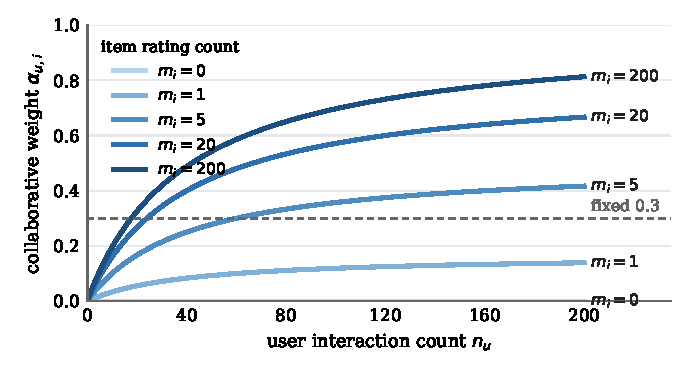
\includegraphics[width=0.8\linewidth]{fig_alpha_two_sided}
  \caption{Collaborative weight $\alpha_{u,i} = t^{\mathrm{user}}_u \cdot t^{\mathrm{item}}_i$ against the user's interaction count, one curve per item rating count ($k = 40$, $k' = 5$). The curve for $m_i = 0$ is identically zero; the dashed line is the fixed weight $\alpha = 0.3$.}
  \label{fig:alpha}
\end{figure}

\begin{table}[t]
  \caption{Fusion weights under the constants selected on TripAdvisor ($k=40$, $k'=5$, $k_c=1$). Unless stated, the item is well observed ($m_i = 200$).}
  \label{tab:weights}
  \centering
  \begin{tabular}{lccc}
    \toprule
    Situation & $\alpha$ & $\beta$ & $\gamma$ \\
    \midrule
    New user ($n_u = 0$)                    & 0.00 & 0.00 & 1.00 \\
    $n_u = 10$                              & 0.20 & 0.73 & 0.07 \\
    $n_u = 40$                              & 0.49 & 0.50 & 0.01 \\
    Established user ($n_u = 200$)          & 0.81 & 0.19 & 0.00 \\
    Established user, item with one rating  & 0.14 & 0.86 & 0.00 \\
    Established user, new item ($m_i = 0$)  & 0.00 & 1.00 & 0.00 \\
    \bottomrule
  \end{tabular}
\end{table}

% =====================================================================
\section{Experimental Setup}
\label{sec:setup}

\subsection{Datasets}

Two datasets are used, one from the standard benchmark domain and one from the target domain.

\paragraph{MovieLens 100K}~\cite{harper2015} contains 100{,}000 ratings by 943 users on 1{,}682 films, with genre attributes as content features and age, gender and occupation as demographic attributes. It is included because it is the standard benchmark for this class of comparison, and because every method under test was designed with it in mind.

\paragraph{TripAdvisor} is the public corpus scraped and released by Mr\'azov\'a and Beh\'un~\cite{mrazova2023}: 3.1~million reviews of 3{,}260 hotels. Reviews without an overall rating are discarded and users with fewer than five reviews are removed, leaving 382{,}279 ratings by 50{,}009 users on 3{,}131 hotels. Content features are TF-IDF vectors over the hotel's star class, amenities, languages, size band and region. The corpus carries no age, gender or occupation; the demographic component uses the reviewer's home region and most frequent trip type, so the demographic signal is weaker here than on MovieLens, and we say so where it matters. To our knowledge this is the only public hotel corpus that provides, at once, user identifiers, item attributes and some user-side profile information, the three inputs the method requires; the larger HotelRec corpus, for instance, carries no user profile at all.

\subsection{Cold-Start Simulation}

Every MovieLens user has at least 20 ratings and most TripAdvisor users have few, so cold start is induced by the same protocol on both datasets, following Schein et al.~\cite{schein2002}. Per seed:
\begin{itemize}
  \item \textbf{New items.} 20\% of items are drawn at random and \emph{all} of their ratings are moved to the held-out split, so these items have $m_i = 0$ in training.
  \item \textbf{Cold users.} 30\% of users are drawn at random and only their first $n$ ratings in chronological order are kept in training, with $n$ drawn uniformly from $\{0,\dots,19\}$.
  \item The remaining users contribute 20\% of their ratings to the held-out split.
\end{itemize}
The held-out split is divided in half into validation and test. Test rows are grouped by the user's training count into \emph{cold} ($n_u < 5$), \emph{cool} ($5 \le n_u < 20$) and \emph{warm} ($n_u \ge 20$), plus a separate \emph{new-item} group. Averaged over seeds, the MovieLens test split holds 10{,}374 new-item rows and 658 / 2{,}060 / 5{,}242 cold / cool / warm rows; TripAdvisor holds 38{,}415 and 19{,}001 / 11{,}936 / 669.

\subsection{Protocol}

Every result is the mean over ten seeds, each a different random split. A temporal split, as used in companion studies of the same platform, was considered and rejected for this experiment: in the final year of the TripAdvisor corpus almost no hotel receives its first review, so a time-based test set contains too few items with $m_i = 0$ to measure new-item exposure at all; holding out 20\% of items is the only way to create enough of them. All methods are tuned by the identical procedure: a grid search on the validation split, selecting by RMSE. The test split is never consulted during tuning. The grid for the proposed rule is $k \in \{5,10,20,40,80,160\}$, $k' \in \{5,20,50,100,200,400\}$ and $k_c \in \{1,3,10,30\}$. Because the constants are re-selected per seed, we report the modal choice: $(k,k',k_c) = (80,5,10)$ on MovieLens and $(40,5,1)$ on TripAdvisor, the latter in eight of ten seeds. The upper end of the $k'$ grid was never selected on either dataset.

\subsection{Metrics}

Rating accuracy is reported as RMSE and MAE on the test rows. Ranking quality is reported as NDCG@10, computed by ranking every item the user has not rated in training, that is over the \emph{full catalogue}, following Krichene and Rendle~\cite{krichene2020}. Ranking inside a sampled candidate set of items the user happened to rate inflates all methods and, critically, never contains an item with $m_i = 0$, so it cannot measure item-side cold start at all. On TripAdvisor the ranking metrics are computed on a random sample of 2{,}000 test users per seed, since scoring all 50{,}009 users against 3{,}131 hotels for seventeen methods is prohibitive; rating metrics use every test row.

Two beyond-accuracy measures are reported. Cov@10 is the fraction of the catalogue that appears in at least one top-10 list. New@10 is the fraction of top-10 slots occupied by items with $m_i = 0$; it is the direct measure of whether a method can surface an item nobody has rated. Differences between the proposed method and each baseline are tested with a two-sided Wilcoxon signed-rank test over the ten per-seed values; with ten seeds the smallest attainable $p$ is $0.002$.

\subsection{Baselines}

Four single-paradigm references (Popularity, Demographic-only, Content-only, CF-only), three fixed-weight hybrids over the same three components with $\alpha \in \{0.3, 0.5, 0.7\}$ and the remainder split 70/30 between content and demographic, and four published hybrids~\cite{tarek2022,do2020,ohwsf2025,slarec2026} reimplemented inside the harness. The reimplementations are adaptations rather than reproductions: each original uses a different dataset, split and metric, so their published numbers are not comparable to ours and are not quoted. Each is tuned by the same validation grid search as the proposed method.

% =====================================================================
\section{Results}
\label{sec:results}

\subsection{Overall}

Table~\ref{tab:overall} reports the mean over ten seeds on both datasets.

\begin{table}[t]
  \caption{Overall results, mean over ten seeds. Best value per column in bold. New@10 is the fraction of top-10 slots filled by items with no training ratings.}
  \label{tab:overall}
  \centering
  \small
  \setlength{\tabcolsep}{4pt}
  \begin{tabular}{l ccccc ccccc}
    \toprule
    & \multicolumn{5}{c}{MovieLens 100K} & \multicolumn{5}{c}{TripAdvisor} \\
    \cmidrule(lr){2-6}\cmidrule(lr){7-11}
    Method & RMSE & MAE & NDCG & Cov & New & RMSE & MAE & NDCG & Cov & New \\
    \midrule
    Popularity        & 1.0806 & 0.8893 & 0.0360 & 0.022 & 0.0000 & 0.9459 & 0.7183 & 0.0026 & 0.004 & 0.0000 \\
    Demographic-only  & 1.0829 & 0.8908 & 0.0401 & 0.057 & 0.0000 & 0.9477 & 0.7205 & 0.0031 & 0.030 & 0.0000 \\
    Content-only      & 1.0215 & 0.8159 & 0.0398 & 0.117 & 0.0016 & 0.9175 & 0.7059 & 0.0030 & 0.042 & 0.0008 \\
    CF-only (SVD++)   & 1.0306 & 0.8290 & 0.0447 & 0.157 & 0.0000 & 0.9200 & 0.7088 & \textbf{0.0033} & \textbf{0.119} & 0.0000 \\
    \midrule
    Fixed $\alpha=0.3$ & 1.0161 & 0.8204 & 0.0443 & 0.072 & 0.0000 & \textbf{0.9104} & \textbf{0.7014} & 0.0029 & 0.029 & 0.0000 \\
    Fixed $\alpha=0.5$ & 1.0169 & 0.8205 & 0.0455 & 0.088 & 0.0000 & 0.9117 & 0.7024 & 0.0029 & 0.040 & 0.0000 \\
    Fixed $\alpha=0.7$ & 1.0204 & 0.8224 & 0.0457 & 0.111 & 0.0000 & 0.9141 & 0.7044 & 0.0029 & 0.061 & 0.0000 \\
    \midrule
    Tarek et al.~\cite{tarek2022}   & 1.0206 & 0.8289 & 0.0424 & 0.082 & 0.0000 & 0.9135 & \textbf{0.7014} & 0.0028 & 0.013 & 0.0000 \\
    Do et al.~\cite{do2020}         & 1.0192 & 0.8177 & 0.0432 & 0.093 & 0.0000 & 0.9125 & 0.7031 & 0.0029 & 0.038 & 0.0000 \\
    OHWSF~\cite{ohwsf2025}          & 1.0305 & 0.8289 & 0.0443 & 0.155 & 0.0000 & 0.9163 & 0.7052 & 0.0030 & 0.077 & 0.0000 \\
    SL-ARec~\cite{slarec2026}       & 1.0155 & 0.8159 & \textbf{0.0504} & \textbf{0.166} & 0.0031 & 0.9109 & 0.7020 & 0.0030 & 0.035 & 0.0001 \\
    \midrule
    \textbf{Proposed} & \textbf{1.0148} & \textbf{0.8111} & 0.0480 & 0.147 & \textbf{0.0118} & 0.9151 & 0.7060 & 0.0029 & 0.046 & \textbf{0.0024} \\
    \bottomrule
  \end{tabular}
\end{table}

Three observations hold on both datasets. First, nine of the eleven baselines, that is every method except Content-only and SL-ARec, have a New@10 of exactly zero: across ten seeds and thousands of users they never place an item with $m_i = 0$ in a top-10 list. Second, the proposed rule has the highest New@10 by a wide margin: $0.0118$ against $0.0031$ for SL-ARec on MovieLens, and $0.0024$ against $0.0001$ on TripAdvisor. Third, this is achieved without a loss in ranking quality: on MovieLens the proposed rule is second on NDCG@10, behind SL-ARec, and on TripAdvisor all twelve methods lie between $0.0026$ and $0.0033$ and are statistically indistinguishable (Section~\ref{sec:significance}).

On rating error the two datasets disagree. On MovieLens the proposed rule attains the lowest RMSE and MAE of the twelve methods. On TripAdvisor it does not: the fixed $\alpha = 0.3$ hybrid is best at $0.9104$, and the proposed rule, at $0.9151$, ranks ninth. We return to this in Section~\ref{sec:discussion}; here we note only that the nine hybrid configurations span a range of $0.006$~RMSE on a five-point scale.

\subsection{By Cold-Start Group}

Table~\ref{tab:groups} breaks the results down by the user's training count. On MovieLens, where ranking metrics are large enough to separate methods, the pattern matches the design: for cold users the proposed rule is the best of all twelve on NDCG@10, because $\alpha$ is near zero there and the ranking is carried by the content and demographic components, while CF-only is among the weakest. For warm users CF-only improves by a factor of nearly three over its cold-user figure, and the proposed rule tracks it upward while remaining behind SL-ARec, whose LightGCN component is stronger on dense data.

\begin{table}[t]
  \caption{Results by cold-start group, mean over ten seeds. Left: NDCG@10 by user group on MovieLens. Right: RMSE by group on TripAdvisor, including the new-item group.}
  \label{tab:groups}
  \centering
  \small
  \setlength{\tabcolsep}{4pt}
  \begin{tabular}{l ccc cccc}
    \toprule
    & \multicolumn{3}{c}{MovieLens, NDCG@10} & \multicolumn{4}{c}{TripAdvisor, RMSE} \\
    \cmidrule(lr){2-4}\cmidrule(lr){5-8}
    Method & Cold & Cool & Warm & New item & Cold & Cool & Warm \\
    \midrule
    Popularity        & 0.0257 & 0.0205 & 0.0479 & 0.9691 & 0.9242 & 0.9081 & 0.8535 \\
    Demographic-only  & 0.0297 & \textbf{0.0240} & 0.0524 & 0.9691 & 0.9298 & 0.9105 & 0.8484 \\
    Content-only      & 0.0297 & 0.0214 & 0.0537 & 0.9449 & 0.9017 & 0.8586 & 0.7635 \\
    CF-only (SVD++)   & 0.0220 & 0.0224 & 0.0629 & 0.9392 & 0.9117 & 0.8762 & 0.7925 \\
    Fixed $\alpha=0.3$ & 0.0274 & 0.0223 & 0.0614 & \textbf{0.9372} & \textbf{0.8945} & 0.8536 & 0.7626 \\
    Fixed $\alpha=0.5$ & 0.0264 & 0.0227 & 0.0636 & 0.9375 & 0.8967 & 0.8566 & 0.7656 \\
    Tarek et al.      & 0.0272 & 0.0227 & 0.0578 & 0.9394 & 0.8972 & 0.8601 & 0.7779 \\
    Do et al.         & 0.0274 & 0.0223 & 0.0595 & 0.9390 & 0.8968 & 0.8566 & 0.7630 \\
    OHWSF             & 0.0217 & 0.0220 & 0.0624 & 0.9389 & 0.9046 & 0.8666 & 0.7770 \\
    SL-ARec           & 0.0298 & 0.0231 & \textbf{0.0717} & 0.9377 & 0.8954 & 0.8537 & \textbf{0.7621} \\
    \textbf{Proposed} & \textbf{0.0306} & 0.0230 & 0.0673 & 0.9449 & 0.8959 & \textbf{0.8536} & 0.7634 \\
    \bottomrule
  \end{tabular}
\end{table}

The TripAdvisor columns show the price of the content-only rule for unrated items. On the new-item group the proposed rule's RMSE coincides with Content-only's ($0.9449$), by construction, and is $0.008$ worse than the best fixed-weight hybrid, which still blends in a demographic estimate for those rows. The rule therefore trades a small amount of rating accuracy on new items for the ability to rank them at all; on the cold, cool and warm groups the proposed rule is within $0.002$ of the best method.

\subsection{Ablation}
\label{sec:ablation}

Table~\ref{tab:ablation} isolates the two design choices of Section~\ref{sec:method}. Each variant keeps everything else fixed and is re-tuned by the same grid search.

\begin{table}[t]
  \caption{Ablation of the fusion rule, mean over ten seeds. Rows 2--4 keep the content-only rule for unrated items and change only how $\alpha$ is formed; row 5 keeps the product and removes that rule.}
  \label{tab:ablation}
  \centering
  \small
  \begin{tabular}{l ccc ccc}
    \toprule
    & \multicolumn{3}{c}{MovieLens 100K} & \multicolumn{3}{c}{TripAdvisor} \\
    \cmidrule(lr){2-4}\cmidrule(lr){5-7}
    Variant & RMSE & NDCG@10 & New@10 & RMSE & NDCG@10 & New@10 \\
    \midrule
    Proposed: $\alpha = t^{\mathrm{user}} \cdot t^{\mathrm{item}}$ & 1.0148 & 0.0480 & \textbf{0.0118} & 0.9151 & 0.0029 & \textbf{0.0024} \\
    $\alpha = t^{\mathrm{user}}$ (user side only)                   & 1.0173 & 0.0456 & 0.0074 & \textbf{0.9132} & 0.0028 & 0.0000 \\
    $\alpha = (t^{\mathrm{user}} + t^{\mathrm{item}})/2$            & 1.0150 & 0.0474 & 0.0075 & 0.9142 & 0.0028 & 0.0000 \\
    Product, without content-only rule for $m_i = 0$                & \textbf{1.0114} & 0.0476 & 0.0011 & 0.9116 & 0.0029 & 0.0001 \\
    \bottomrule
  \end{tabular}
\end{table}

\begin{figure}[t]
  \centering
  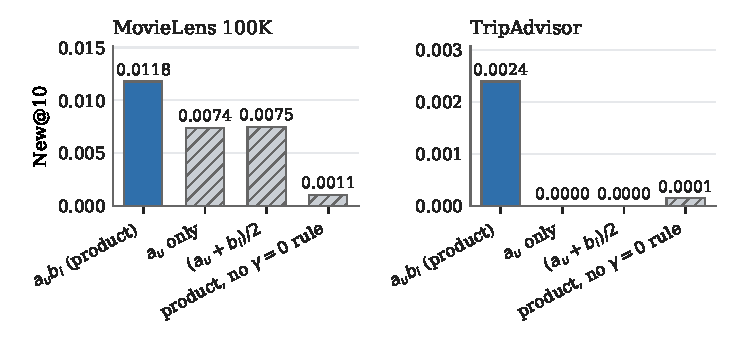
\includegraphics[width=0.95\linewidth]{fig_newitem_ablation}
  \caption{New@10 of the four variants of Table~\ref{tab:ablation}, mean over ten seeds. On TripAdvisor only the product combined with the content-only rule places any unrated hotel in a top-10 list.}
  \label{fig:ablation}
\end{figure}

Fig.~\ref{fig:ablation} shows the New@10 column of the table as bars.

\paragraph{Product versus user-side factor.} Replacing the product by the user-side factor alone, which is the form used by Melville et al.\ and Do et al.~\cite{melville2002,do2020}, lowers New@10 from $0.0118$ to $0.0074$ on MovieLens and from $0.0024$ to exactly $0.0000$ on TripAdvisor. The TripAdvisor outcome is the one the construction predicts: an established user there has $t^{\mathrm{user}}$ close to one, so a user-side rule hands the full collaborative weight to a hotel the CF model has never seen, and content similarity never gets to rank it. On MovieLens the user-side variant is also worse on RMSE and NDCG@10 (10/10 seeds on all three measures, $p = 0.002$).

\paragraph{Product versus mean.} Averaging the two factors behaves like the user-side rule: it retains some New@10 on MovieLens ($0.0075$) but none on TripAdvisor. A mean cannot drive $\alpha$ to zero when only one side is empty, which is exactly the two-sided case.

\paragraph{Content-only rule for unrated items.} Removing this rule, while keeping the product, lowers New@10 by an order of magnitude on both datasets, from $0.0118$ to $0.0011$ and from $0.0024$ to $0.0001$, and improves RMSE slightly ($1.0114$ and $0.9116$). This is the trade-off already visible in Table~\ref{tab:groups}: the demographic component carries a little rating-scale accuracy on new items but returns a near-constant value across them, so it cannot order them, and blending it in pushes all of them below the top-10 cut-off.

The two choices are therefore complementary. The product guarantees that an unrated item is not handed to the collaborative model; the content-only rule guarantees that, once handed to the remaining components, it is scored by the one that can distinguish it from other unrated items. Either alone is insufficient.

\subsection{Significance}
\label{sec:significance}

Table~\ref{tab:wilcoxon} reports the Wilcoxon signed-rank test over the ten per-seed values of the proposed rule against each baseline and ablation variant.

\begin{table}[t]
  \caption{Wilcoxon signed-rank test over ten seeds. ``Wins'' counts seeds on which the proposed rule is better. Entries with $p \ge 0.05$ are not significant.}
  \label{tab:wilcoxon}
  \centering
  \small
  \setlength{\tabcolsep}{3.5pt}
  \begin{tabular}{l cc cc cc cc}
    \toprule
    & \multicolumn{4}{c}{MovieLens 100K} & \multicolumn{4}{c}{TripAdvisor} \\
    \cmidrule(lr){2-5}\cmidrule(lr){6-9}
    & \multicolumn{2}{c}{RMSE} & \multicolumn{2}{c}{New@10} & \multicolumn{2}{c}{RMSE} & \multicolumn{2}{c}{New@10} \\
    Compared with & Wins & $p$ & Wins & $p$ & Wins & $p$ & Wins & $p$ \\
    \midrule
    CF-only (SVD++)      & 10/10 & 0.002 & 10/10 & 0.002 & 10/10 & 0.002 & 10/10 & 0.002 \\
    Content-only         & 10/10 & 0.002 & 10/10 & 0.002 & 10/10 & 0.002 & 10/10 & 0.002 \\
    Fixed $\alpha=0.3$   &  9/10 & 0.006 & 10/10 & 0.002 &  0/10 & 0.002 & 10/10 & 0.002 \\
    Tarek et al.         & 10/10 & 0.002 & 10/10 & 0.002 &  1/10 & 0.004 & 10/10 & 0.002 \\
    Do et al.            & 10/10 & 0.002 & 10/10 & 0.002 &  0/10 & 0.002 & 10/10 & 0.002 \\
    OHWSF                & 10/10 & 0.002 & 10/10 & 0.002 &  9/10 & 0.004 & 10/10 & 0.002 \\
    SL-ARec              &  6/10 & 0.275 & 10/10 & 0.002 &  0/10 & 0.002 & 10/10 & 0.002 \\
    \midrule
    $\alpha = t^{\mathrm{user}}$ only          & 10/10 & 0.002 & 10/10 & 0.002 & 0/10 & 0.002 & 10/10 & 0.002 \\
    $\alpha$ = mean of factors                 &  9/10 & 0.049 &  9/10 & 0.004 & 0/10 & 0.002 & 10/10 & 0.002 \\
    Without content-only rule                  &  0/10 & 0.002 & 10/10 & 0.002 & 0/10 & 0.002 & 10/10 & 0.002 \\
    \bottomrule
  \end{tabular}
\end{table}

On New@10 the advantage is significant against every baseline and every ablation variant on both datasets, in all cases $10/10$ seeds except the mean-of-factors variant on MovieLens ($9/10$, $p = 0.004$). On RMSE the picture is split: on MovieLens the proposed rule is significantly better than every baseline except SL-ARec, where six wins out of ten is indistinguishable from chance and no claim is made; on TripAdvisor it is significantly \emph{worse} than the fixed-weight and published hybrids, by $0.002$ to $0.005$. On NDCG@10, not tabulated, no pair of methods differs significantly on TripAdvisor ($p \ge 0.275$ in every comparison), whereas on MovieLens the proposed rule beats every baseline except SL-ARec at $p \le 0.002$.

\subsection{Why Rating Error Does Not Discriminate on Hotel Data}
\label{sec:discussion}

The TripAdvisor RMSE result deserves explanation rather than concealment, because it reverses the MovieLens result. Two measurements account for it.

First, the errors of the collaborative and content components are almost perfectly correlated on this dataset: the Pearson correlation between the residuals $s^{\mathrm{CF}}_{u,i} - r_{u,i}$ and $s^{\mathrm{CB}}_{u,i} - r_{u,i}$ over the test rows is $0.975$, averaged over the ten seeds, and never below $0.974$ on any of them. Two predictors that err on the same rows in the same direction gain almost nothing from being averaged, whatever the weights. Sweeping the collaborative weight from $0$ to $0.4$ at a fixed demographic weight moves RMSE by only $0.001$, which is why nine hybrid configurations, four of them published methods, land within $0.006$ of one another in Table~\ref{tab:overall}. On this data RMSE simply does not separate fusion rules.

Second, the evidence counts on TripAdvisor are small: the median test user has four training ratings and, because 20\% of hotels are held out entirely, the median test row has an item count of zero. The product rule consequently assigns a mean collaborative weight of only $0.045$ across the test split, while the sweep places the RMSE-optimal value near $0.2$. The rule's premise, that CF is unreliable at low counts, is sound for ranking, where CF genuinely cannot order unseen items, but overly cautious for rating error, where SVD++ still estimates the user and item biases from a handful of ratings. This is the mechanism behind the $0.002$--$0.005$ RMSE deficit, and it is also why the variance that side information can explain is small on this corpus: a one-way decomposition of the rating variance attributes 28.0\% to the user, 12.7\% to the hotel, and under 1\% to the hotel's region, the trip type or the reviewer's region combined.

The practical reading is the one McNee et al.\ argued for~\cite{mcnee2006}: when rating error is saturated, as it is here, the criterion that still distinguishes fusion rules is a beyond-accuracy one. On this dataset that criterion is whether a newly listed hotel can be recommended at all, and on that criterion the difference between the rules is not a few thousandths but the difference between a non-zero rate and zero.

% =====================================================================
\section{Threats to Validity}
\label{sec:threats}

\paragraph{Domain and data.} MovieLens is a film benchmark, and the TripAdvisor corpus consists of explicit review ratings rather than booking logs. Neither carries price or availability, so the knowledge-based pre-filter of Section~\ref{sec:problem} is absent from every reported number. The conclusions concern the weighting rule, not the deployed platform.

\paragraph{Demographic signal on TripAdvisor.} The corpus has no age, gender or occupation; the demographic component uses home region and trip type, which explain under 1\% of rating variance. The weak demographic results on TripAdvisor may understate what a richer profile would give. They do not affect the New@10 findings, which depend on the content component.

\paragraph{Magnitude of New@10.} The absolute rates ($0.0118$ and $0.0024$) are small, because 20\% of the catalogue is unrated and the metric counts top-10 slots. The claim is comparative: nine of eleven baselines, and all of the ablation variants on TripAdvisor, attain exactly zero. We do not measure whether the surfaced new items are the ones the user would have preferred among new items, which would require relevance judgements on unrated hotels that the data do not contain; we only verify that NDCG@10 does not fall.

\paragraph{Ranking sample on TripAdvisor.} Ranking metrics there use 2{,}000 sampled users per seed. With ten seeds this covers 20{,}000 user--catalogue rankings, but the small NDCG values ($\approx 0.003$) are close to the resolution of the sample and should be read as ``indistinguishable'' rather than as a ranking of methods.

\paragraph{Reimplemented baselines.} The four published methods are adaptations constrained to this harness and tuned by our grid search. Their numbers characterise the \emph{idea} under common conditions, not the original systems.

\paragraph{Per-seed tuning.} The three constants are re-selected on each split; the modal choice differs between datasets. A deployed system would fix them once, and the reported numbers are an upper bound on what a single fixed triple attains.

\paragraph{Simulated rather than temporal cold start.} New items and cold users are created by random hold-out, not by a time split. The simulation is the only protocol that yields enough unrated items to measure New@10, but it ignores the order in which hotels actually appear, and a hotel held out at random is not a hotel that was listed last; a temporal evaluation of the rule on booking logs remains to be done.

\paragraph{Reproducibility.} The code, the per-seed result files and the run manifests behind every table are available at \url{https://github.com/phucdhcoder19/stayreco-experiment}.

% =====================================================================
\section{Conclusion}

Under two-sided cold start the mixing weight of a hybrid recommender must depend on the evidence available on both axes. Making the collaborative weight the product of a user-side and an item-side shrinkage factor enforces this directly: either side lacking data removes the collaborative term entirely. Scoring an unrated item by content alone then lets the one component that can distinguish new items from each other decide their rank.

On a film benchmark and on a corpus of 382{,}279 hotel ratings, with ten random splits each and full-catalogue ranking, the resulting rule is the only configuration among twelve in which newly listed items reach the top-10 at a non-negligible rate; nine baselines never surface such an item, and replacing the product by a user-side factor or by a mean of the two factors reduces the rate to zero on the hotel data. The rule achieves the lowest rating error on MovieLens but not on TripAdvisor, where all hybrid configurations lie within $0.006$~RMSE because the collaborative and content errors are correlated at $0.97$. We report both outcomes, and read them together: where rating error is saturated, the ability to expose new items is the criterion on which fusion rules should be chosen.

Future work includes evaluation on booking logs once the platform accumulates them, a relevance-aware measure of new-item exposure, estimating the three constants from component error variances rather than by grid search, and bringing the knowledge-based pre-filter into the evaluated pipeline.

\subsubsection*{Acknowledgements.} This work was carried out as a capstone project (FA26SE056) at FPT University, Ho Chi Minh City. We thank Mr\'azov\'a and Beh\'un for making the TripAdvisor corpus publicly available. This work received no external funding.

\subsubsection*{Disclosure of Interests.} The authors have no competing interests to declare that are relevant to the content of this article.

\subsubsection*{Declaration on Generative AI.} During the preparation of this work, the authors used Claude (Anthropic) to draft and revise text, to check the reported numbers against the result files, to generate the figures from those files, and to write parts of the experiment code, which the authors reviewed and ran. After using this tool, the authors reviewed and edited the content and take full responsibility for the publication's content.

% =====================================================================
%  Danh mục tài liệu viết thẳng vào file (định dạng splncs04) để không cần
%  references.bib / splncs04.bst. Thứ tự theo bảng chữ cái tác giả.
\begin{thebibliography}{8}

\bibitem{bernardi2015}
Bernardi, L., Kamps, J., Kiseleva, J., M{\"u}ller, M.J.I.: The continuous cold start problem in e-commerce recommender systems. In: Proceedings of the 2nd Workshop on New Trends on Content-Based Recommender Systems (CBRecSys). CEUR Workshop Proceedings, vol. 1448, pp. 30--33 (2015)

\bibitem{burke2002}
Burke, R.: Hybrid recommender systems: survey and experiments. User Modeling and User-Adapted Interaction \textbf{12}(4), 331--370 (2002)

\bibitem{slarec2026}
{\c{C}}ak{\i}r, M.E., {\c{C}}etinkaya, Z., Horasan, F., Yurttakal, A.H.: Adaptive weighting-based hybrid recommender system: self-learning adaptive recommendation (SL-ARec). PeerJ Computer Science \textbf{12}, e3856 (2026)

\bibitem{claypool1999}
Claypool, M., Gokhale, A., Miranda, T., Murnikov, P., Netes, D., Sartin, M.: Combining content-based and collaborative filters in an online newspaper. In: Proceedings of the ACM SIGIR Workshop on Recommender Systems (1999)

\bibitem{do2020}
Do, H.-Q., Le, T.-H., Yoon, B.: Dynamic weighted hybrid recommender systems. In: Proceedings of the 22nd International Conference on Advanced Communication Technology (ICACT), pp. 644--650 (2020)

\bibitem{dacrema2019}
Ferrari Dacrema, M., Cremonesi, P., Jannach, D.: Are we really making much progress? A worrying analysis of recent neural recommendation approaches. In: Proceedings of the 13th ACM Conference on Recommender Systems (RecSys), pp. 101--109 (2019)

\bibitem{harper2015}
Harper, F.M., Konstan, J.A.: The MovieLens datasets: history and context. ACM Transactions on Interactive Intelligent Systems \textbf{5}(4), 1--19 (2015)

\bibitem{lightgcn2020}
He, X., Deng, K., Wang, X., Li, Y., Zhang, Y., Wang, M.: LightGCN: simplifying and powering graph convolution network for recommendation. In: Proceedings of the 43rd International ACM SIGIR Conference on Research and Development in Information Retrieval, pp. 639--648 (2020)

\bibitem{herlocker2004}
Herlocker, J.L., Konstan, J.A., Terveen, L.G., Riedl, J.T.: Evaluating collaborative filtering recommender systems. ACM Transactions on Information Systems \textbf{22}(1), 5--53 (2004)

\bibitem{kaminskas2016}
Kaminskas, M., Bridge, D.: Diversity, serendipity, novelty, and coverage: a survey and empirical analysis of beyond-accuracy objectives in recommender systems. ACM Transactions on Interactive Intelligent Systems \textbf{7}(1), 1--42 (2016)

\bibitem{koren2008}
Koren, Y.: Factorization meets the neighborhood: a multifaceted collaborative filtering model. In: Proceedings of the 14th ACM SIGKDD International Conference on Knowledge Discovery and Data Mining, pp. 426--434 (2008)

\bibitem{krichene2020}
Krichene, W., Rendle, S.: On sampled metrics for item recommendation. In: Proceedings of the 26th ACM SIGKDD International Conference on Knowledge Discovery and Data Mining, pp. 1748--1757 (2020)

\bibitem{lops2011}
Lops, P., de Gemmis, M., Semeraro, G.: Content-based recommender systems: state of the art and trends. In: Ricci, F., Rokach, L., Shapira, B., Kantor, P.B. (eds.) Recommender Systems Handbook, pp. 73--105. Springer (2011)

\bibitem{mcnee2006}
McNee, S.M., Riedl, J., Konstan, J.A.: Being accurate is not enough: how accuracy metrics have hurt recommender systems. In: CHI '06 Extended Abstracts on Human Factors in Computing Systems, pp. 1097--1101 (2006)

\bibitem{melville2002}
Melville, P., Mooney, R.J., Nagarajan, R.: Content-boosted collaborative filtering for improved recommendations. In: Proceedings of the 18th National Conference on Artificial Intelligence (AAAI), pp. 187--192 (2002)

\bibitem{mrazova2023}
Mr{\'a}zov{\'a}, I., Beh{\'u}n, M.: Graph neural networks for hotel recommendation and quality assessment. In: Proceedings of the 23rd Conference on Information Technologies -- Applications and Theory (ITAT 2023). CEUR Workshop Proceedings, vol. 3498, pp. 67--75 (2023)

\bibitem{ohwsf2025}
Muhammad, M., Gunardi, Danardono, Rosadi, D.: Optimization hybrid weighted switching filtering (OHWSF) using SVD and SVD++ for addressing data sparsity. International Journal of Advances in Intelligent Informatics \textbf{11}(3), 533 (2025)

\bibitem{pazzani1999}
Pazzani, M.J.: A framework for collaborative, content-based and demographic filtering. Artificial Intelligence Review \textbf{13}(5--6), 393--408 (1999)

\bibitem{rendle2020}
Rendle, S., Krichene, W., Zhang, L., Anderson, J.: Neural collaborative filtering vs. matrix factorization revisited. In: Proceedings of the 14th ACM Conference on Recommender Systems (RecSys), pp. 240--248 (2020)

\bibitem{schein2002}
Schein, A.I., Popescul, A., Ungar, L.H., Pennock, D.M.: Methods and metrics for cold-start recommendations. In: Proceedings of the 25th Annual International ACM SIGIR Conference on Research and Development in Information Retrieval, pp. 253--260 (2002)

\bibitem{tarek2022}
Tarek, I.H.M., Munna, F.U., Mojumder, A.T.M.T.H., Rahman, M.M., Hossain, M.S., Andersson, K.: A hybrid hotel recommendation using collaborative, content based and knowledge based approach. In: Intelligent Computing \& Optimization. Lecture Notes in Networks and Systems, pp. 1049--1057. Springer (2022)

\end{thebibliography}

\end{document}
